\chapter{Introduction}
\label{chp:intro}

% large
Massive text data, which has recently become available, allows for building \textit{document classification} models in various domains including news, scientific articles, medical records, political bills, online reviews and social media posts.
Document classifiers, which automatically classify documents into categories, have been widely used for surveillance and diagnosis systems in public health~\cite{lamb2013separating, de2016discovering, huang2019can, zhu2019detecting}, sentiment analysis and user attribute inference in computational social science~\cite{rosenthal2011age, yang2016hierarchical, huang2017exploring, heindorf2019debiasing}, user modeling in personalization~\cite{tang2015learning, wu2016personalized, huang2019neuraluser, pan2019social} and much more. 
The reliability of document classifiers is crucial to the applied domains.


Language varies across document metadata including demographic and temporal factors making document classifiers less robust and generalized. 
However, models for document classification, the automatic categorization of documents into categories, typically ignore metadata attributes of documents. 
\textit{Metadata}, implicitly embedded in documents such as time, author demographic attributes (gender, age, location) and user histories, can impact on the reliability of document classifiers.
On the one hand, users are generating new contents as well as new ways to express their opinions leading to change in word usage and sense over time, and different demographic groups are using written language as a marker of their own social and community identities causing expression ambiguities.
For instance, emoji have been reshaping how people express opinions and sentiments over the years~\cite{felbo2017using}, males and females will use the same words to express opposite sentiment~\cite{volkova2013exploring}, people may perceive ``corona'' more likely as a beer brand in 2019 vs. a virus name in 2020, and users use different words to express the same sentiment and use the same words to express different meanings~\cite{oba2019modeling}. % examples
On the other hand, document classifiers are generally trained without considering those language variations resulting in instability of classifiers or fairness issues: existing research has pointed out failures of existing classifiers because of ignoring time- and demographic- sensitive attributes in social media data~\cite{gayo2011limits, gayo2013predicting}.
We illustrate how the metadata impacts document classifiers in Figure~\ref{chap1:fig:impact}.
% As a result, it is increasingly important to understand, consider and adapt language variations into document classifiers.


\begin{figure}[htp]
\centering
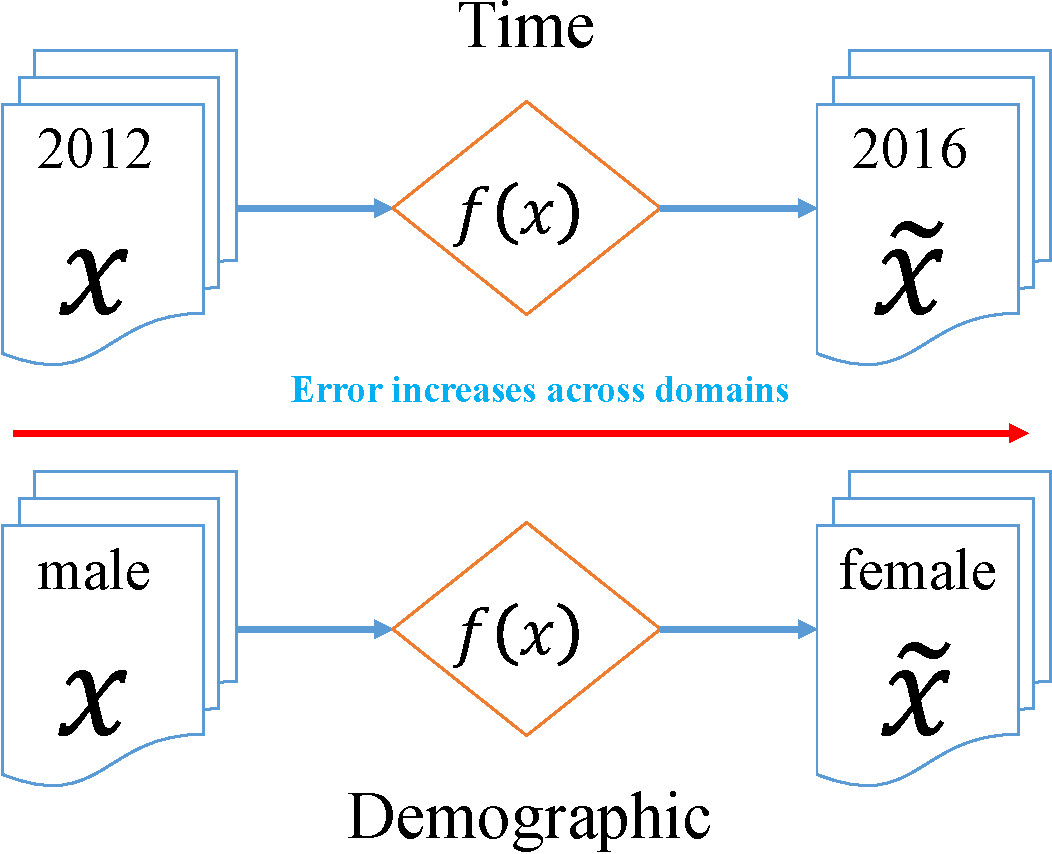
\includegraphics[width=0.60\textwidth]{images/chapter1/metadata_impact.pdf}
\caption{Illustration of how the two metadata will impact on performance of document classifiers. The $\tilde{x}$ indicates the language distributions are different from $x$.}
\label{chap1:fig:impact}
\end{figure}

\section{Contributions and Thesis Overview}

\begin{figure}[htp]
\centering
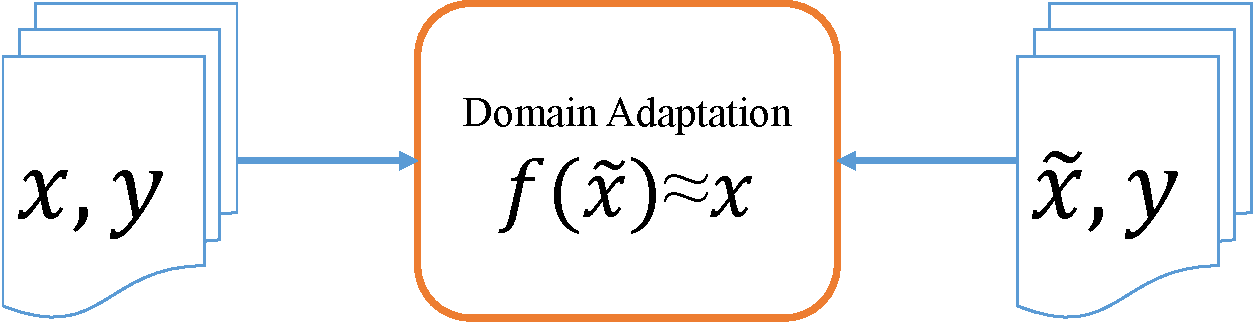
\includegraphics[width=0.70\textwidth]{images/chapter1/da_illu.pdf}
\caption{Illustration of how the domain adaptation works when distributions over $x$ differs in the two sets of domain documents.}
\label{chap1:fig:da}
\end{figure}


In light of these opportunities and challenges, this thesis proposes methods to treat temporality and user factors as domains (2012 vs. 2016; male vs female) and then adapt the metadata into document classifiers using \textit{domain adaptation}.
Domain adaptation is a framework in machine learning that learns variations between source and target domains and enables models trained on the source to be applied the target domain. 


In this thesis, we primarily model two distributions, language probability distribution ($P(x)$) and conditional probability ($P(y|x)$), while we do not model the label distribution, $P(y)$, across domains. Figure~\ref{chap1:fig:da} presents one example of how the concept works: to connect source and target domains when distributions over $x$ are different, domain adaptation learns a function to align distributions between the target and source domains.
In other cases, the conditional probability $P(y|x)$ can changes across domains.
For example, ``fast'' in a document of ``some medical drugs cure patient fast'' can indicate a positive sentiment in a health domain, while a negative sentiment is in a document of ``batteries run fast'' from an electronic domain.
We assume that the label $y$ do not change.

% We propose to treat each variable of individual metadata type as a domain. For example, for the time, we can treat each year or season as a separate domain; for the demographic factors, we can treat male and female as different domains. 

The primary contribution of this thesis is to introduce various novel domain adaptation approaches and demonstrate how they can be applied for training more robust document classifiers towards the metadata.
In this thesis, we take steps towards generalizing and personalizing document classifiers by adapting metadata of documents.
First, we start with background and applications of domain adaptation.
Second, to integrate temporal and user factors into classifiers, this thesis focuses on two types of adaptation: 1) \textit{temporality adaptation} and 2) \textit{user factor adaptation}.
We explore demographic biases of classification models and propose using domain adaptation to reduce biases of document classifiers in the hate speech detection task.
We provide a detailed overview as follows:

\paragraph{Chapter~\ref{chp:background}} summarizes concepts and background of document classification and domain adaptation. We start with a general discussion of the document classification task and introduce classification models that are widely used in this thesis. We then provide the background of domain adaptation and an overview of several existing domain adaptation methods. The chapter initializes discussions of how language varies across temporality and user factors. Finally, we present evaluation metrics of both model performance and fairness.

\paragraph{Chapter~\ref{chp:temporality}} illustrates and summarizes the work we have done in the temporality adaptation. We present two temporality adaptation methods via feature augmentation and diachronic word embedding to learn and model the temporal variations in documents. By integrating the temporal factor into document classifiers, our proposed methods can improve classification performance. This chapter is based on our published work of \cite{huang2018examining, huang2019neural}.

\paragraph{Chapter~\ref{chp:user}} presents our work on user factor adaptation. We propose two approaches to adapt user factors under the multitask learning framework. For the user demographic factor, we first introduce and publicize a new dataset with author-level attributes. We then train a classifier by both demographic attributes and document class predictions under a multitask learning framework aiming to learn domain invariant document representations. Finally, we show user factor adaptation can generalize and improve classification models. To adapt user latent factors in user history, we propose a multitask user embedding model that jointly learns user interests and language usage. We evaluate the user embedding on an intrinsic task, clustering, and an extrinsic task, document classification. Experiments show that the adaptation method can better model semantic variations of the user language usage. This chapter is based on our work of \cite{huang2019neuraluser, huang2020user}.

\paragraph{Chapter~\ref{chp:fairness}} illustrates how user factors can result in demographic biases of document classifiers on the author-level attributes (gender, race, age and location) and presents methods to reduce demographic biases. 
To examine demographic bias, we propose a multilingual hate speech dataset, which each document associates with several author-level attributes. 
The chapter explores classification performance and biases of document classifiers on both English and other languages. 
The improved classification performance by learning demographic-independent document classifiers in Chapter~\ref{chp:user} motivate us to apply the domain adaptation to reduce demographic biases of document classifiers. 
This chapter is based on our published work of \cite{huang2020multilingual}.

\paragraph{Chapter~\ref{chp:conclusion}} concludes the thesis with contributions and suggests future research directions.

\section{Other Research Work}

My research applies machine learning models to solve health issues including suicide ideation analysis, vaccination surveillance, alcoholism diagnosis and COVID-19. 
My work also collects and publicizes new text datasets from online resources, such as Twitter. 
The following will briefly go through the applications with references.

% applications in public health
Social media sites provide a low-cost and fast accessible way to understand public-health-related opinions and behaviors. \cite{huang2017examining, huang2019can} built document classifiers and applied them to examine and analyze behavioral patterns regarding influenza vaccinations from Twitter across three dimensions: temporality (by week and month), geography (by US state and region) and demography (by gender).
Suicide is a leading cause of death worldwide. \cite{huang2017exploring} explored demographic and geographic compositions of suicidal users by conducting text analysis of their posts between 2011 and 2016, which were collected in a novel datasets from Sina Weibo, akin to Twitter.
COVID-19 related information has overwhelmed online social media, however, links of information failed to be rated for its credibility. \cite{broniatowski2020covid, huang2020coronavirus} introduced a Twitter dataset of COVID-19 and found a large increase in the proportion of state-sponsored propaganda among the less credible URLs.

Nonetheless, classification models can face challenges in different scenarios, especially in dialogue and cross-lingual scenarios. \cite{huang2018modeling} explored temporal shifts of user intentions in the alcoholism diagnosis and further demonstrated that temporality can improve classification model performance for medical diagnosis in the dialogue scenario.
Social media provides rich text corpora for different languages, however, the low computational resources of non-English languages prevent mining wider information coverage. 
\cite{huang2019matters} proposed cross-lingual transfer methods that only train sequential classification models on English corpora and apply the models on the other low-resource languages.
